\documentclass[mathserif,11pt]{beamer}
%%%%%%%%%%%%%%%%%%%%%%%%%%%%%%%%%%%%%%%%%%%%%%%%%%%%%%%%%%%%%%%%%%%%%%%%%%%%%%%%%%%%%%%%%%%%%%%%%%%%%%%%%%%%%%%%%%%
% Appearance
\mode<presentation>
{
	\usetheme{CambridgeUS}
	\usecolortheme{whale}
	\setbeamercovered{transparent}
}
% Redefine beamer colors
\definecolor{UoNblue1}{RGB}{0,155,189}
\definecolor{UoNblue2}{RGB}{0,125,168}
\definecolor{UoNblue3}{RGB}{0,86,151}
\definecolor{UoNblue4}{RGB}{27,42,107}
\definecolor{UoNblue5}{RGB}{25,26,79}
% Captions and titles
\setbeamertemplate{caption}{\raggedright\insertcaption} 
\setbeamercolor{frametitle}{fg=UoNblue3}
\setbeamercolor{title}{bg=UoNblue2}

\setbeamercolor{palette primary}{fg=white, bg=UoNblue3}
\setbeamercolor{palette secondary}{fg=white, bg=UoNblue4}
\setbeamercolor{palette tertiary}{fg=white, bg=UoNblue5}
% Outline slide
\setbeamertemplate{section in toc}[circle]
\setbeamerfont{section number projected}{family=\rmfamily,series=\bfseries,size=\normalsize}
\setbeamercolor{section number projected}{bg=UoNblue5,fg=white}
% Itemize list
\setbeamertemplate{itemize item}[circle]
\setbeamertemplate{itemize subitem}[circle]
\setbeamercolor{itemize item}{fg=UoNblue4}
\setbeamercolor{itemize subitemitem}{fg=UoNblue5}
% Title box
\setbeamertemplate{frametitle}{%
	\nointerlineskip%
	\begin{beamercolorbox}[wd=\paperwidth,ht=2.0ex,dp=0.6ex]{frametitle}
		\hspace*{1ex}\insertframetitle%
	\end{beamercolorbox}%
}
%%%%%%%%%%%%%%%%%%%%%%%%%%%%%%%%%%%%%%%%%%%%%%%%%%%%%%%%%%%%%%%%%%%%%%%%%%%%%%%%%%%%%%%%%%%%%%%%%%%%%%%%%%%%%%%%%%%
\usepackage[english]{babel}
% or whatever
\usepackage[latin1]{inputenc}
% or whatever
\usepackage{array} % To vertically center tabular content 
\usepackage{times}
\usepackage[T1]{fontenc}
%\usepackage{eulervm}
%\usepackage{cmbright}
%%%%%%%%%%%%%%%%%%%%%%%%%%%%%%%%%%%%%%%%%%%%%%%%%%%%%%%%%%%%%%%%%%%%%%%%%%%%%%%%%%%%%%%%%%%%%%%%%%%%%%%%%%%%%%%%%%%%
%\usepackage{tikz}
\usepackage{pgfplots}
\usepackage{tikz-3dplot}
\tdplotsetmaincoords{60}{-30}
\tdplotsetrotatedcoords{0}{90}{90}
\pgfplotsset{every axis/.append style={line width=0.5pt},label style={font=\scriptsize},tick label style={font=\scriptsize},x tick label style={/pgf/number format/.cd,fixed,precision=3, set thousands separator={}},z tick label style={/pgf/number format/.cd,fixed,precision=3, set thousands separator={}}}
\usetikzlibrary{shapes,shadows,arrows,backgrounds,patterns,positioning,automata,calc,decorations.markings,decorations.pathreplacing,bayesnet,arrows.meta}
\usepackage{amsmath,amssymb,mathrsfs,amsfonts,amsthm} % for maths
\usepackage{graphicx}
\usepackage{animate}
%\usepackage{subfig}
\usepackage{eucal}    % for curly math letter symbols
\usepackage{amssymb}  % for ams symbols
\usepackage{pifont}
\usepackage{color} %Invoke options usenames,dvipsnames for larger color choice
\usepackage{microtype} % Slightly tweak font spacing for aesthetics
\usepackage{multicol} % Used for the two-column layout of the document
%%%%%%%%%%%%%%%%%%%%%%%%%%%%%%%%%%%%%%%%%%%%%%%%%%%%%%%%%%%%%%%%%%%%%%%%%%%%%%%%%%%%%%%%%%%%%%%%%%%%%%%%%%%%%%%%%%%%
\DeclareSymbolFontAlphabet{\mathcal} {symbols}
\DeclareSymbolFont{symbols}{OMS}{cm}{m}{n}
\DeclareMathAlphabet{\mathbfit}{OML}{cmm}{b}{it}
\newcommand\id{\ensuremath{\mathbbm{1}}} 
\DeclareMathOperator{\E}{\mathbb{E}}
\DeclareMathOperator{\eye}{\mathbb{I}}
\DeclareMathOperator{\zeros}{\mathbb{O}}
\DeclareMathOperator{\tr}{\textrm{tr}}
\DeclareMathOperator{\vc}{\textrm{vec}}
\DeclareMathOperator{\rk}{\textrm{rk}}
\DeclareMathOperator{\ik}{\mathrm{k}}
\DeclareMathOperator{\ip}{\mathrm{p}}
\DeclareMathOperator{\inn}{\mathrm{n}}
\DeclareMathOperator{\im}{\mathrm{m}}
\DeclareMathOperator{\td}{\mathrm{t}}
\DeclareMathOperator{\kd}{\mathrm{k}}
\DeclareMathOperator{\T}{\mathrm{T}}
\DeclareMathOperator{\K}{\mathrm{K}}
%%%%%%%%%%%%%%%%%%%%%%%%%%%%%%%%%%%%%%%%%%%%%%%%%%%%%%%%%%%%%%%%%%%%%%%%%%%%%%%%%%%%%%%%%%%%%%%%%%%%%%%%%%%%%%%%%%%%
\usepackage[backend=bibtex,style=ieee,doi=false,isbn=false,url=false,eprint=false]{biblatex}
\bibliography{bibliography}
\renewcommand*{\bibfont}{\footnotesize}
%%%%%%%%%%%%%%%%%%%%%%%%%%%%%%%%%%%%%%%%%%%%%%%%%%%%%%%%%%%%%%%%%%%%%%%%%%%%%%%%%%%%%%%%%%%%%%%%%%%%%%%%%%%%%%%%%%%%
% Populate title page
\title[AMR in poultry litter] % (optional, use only with long paper titles)
{Antimicrobial resistance in chicken manure heaps: phenomenological modelling}
\author[A. Kadochnikova]{A. Kadochnikova\inst{1}}
\institute[UoN]{\inst{1}
	School of Mathematical Sciences\\
	The University of Nottingham}
\date{18 Mach 2024}
\logo{
\begin{tikzpicture}[overlay,remember picture]
\node[right=0.05cm] at (current page.212){
\includegraphics[height=0.7cm]{UoNlogoFC}};
\end{tikzpicture}}
\begin{document}
\begin{frame}
	\titlepage
\end{frame}
\begin{frame}{Outline}
\tableofcontents[hideallsubsections]
\end{frame}
\section{Our project}
\subsection{Background}
\begin{frame}{Public health threat}
%\begin{columns}
%	\begin{column}{0.5\textwidth}
%	\centering
%		
\includegraphics[width=\textwidth]{Figures/headline_july_2023.png}\\
%		\vspace{0.5cm}
%		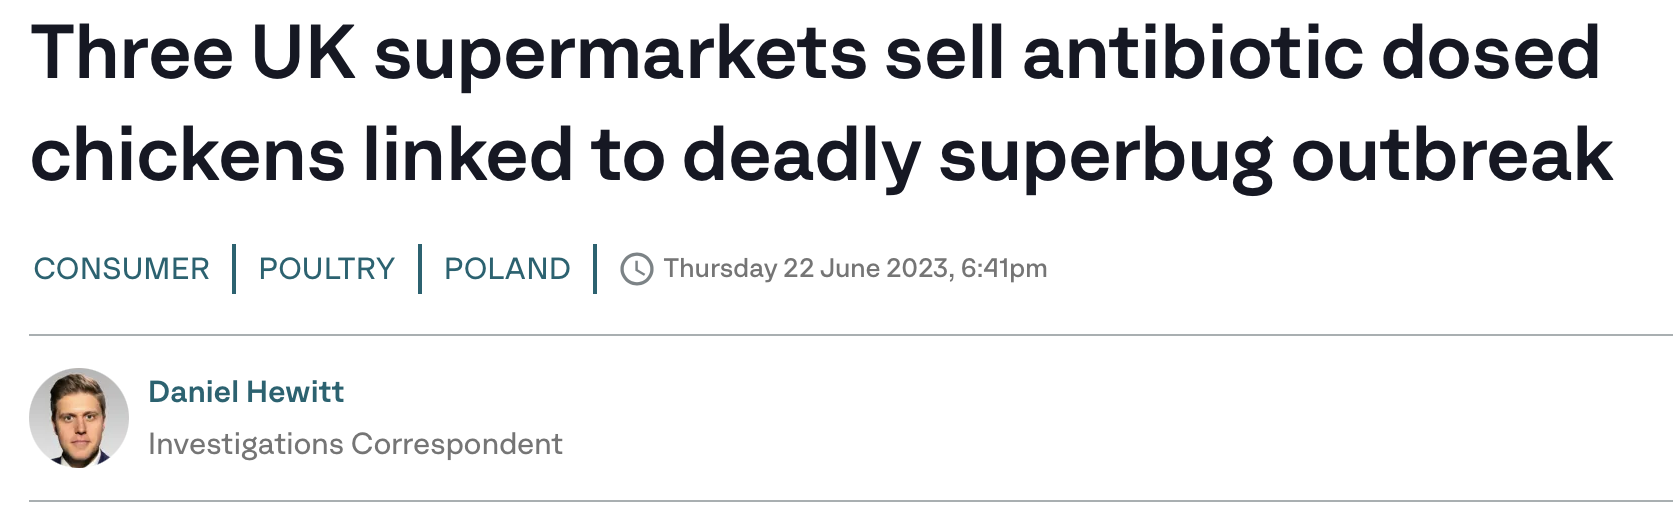
\includegraphics[width=\textwidth]{Figures/headline_itv.png}
%	\end{column}
%	\begin{column}{0.5\textwidth}
%	\centering
%		
\includegraphics[width=\textwidth]{Figures/headline4.png}\\
%		\vspace{0.5cm}
%		
\includegraphics[width=\textwidth]{Figures/headline5.png}\\
%	\end{column}
%\end{columns}
\centering
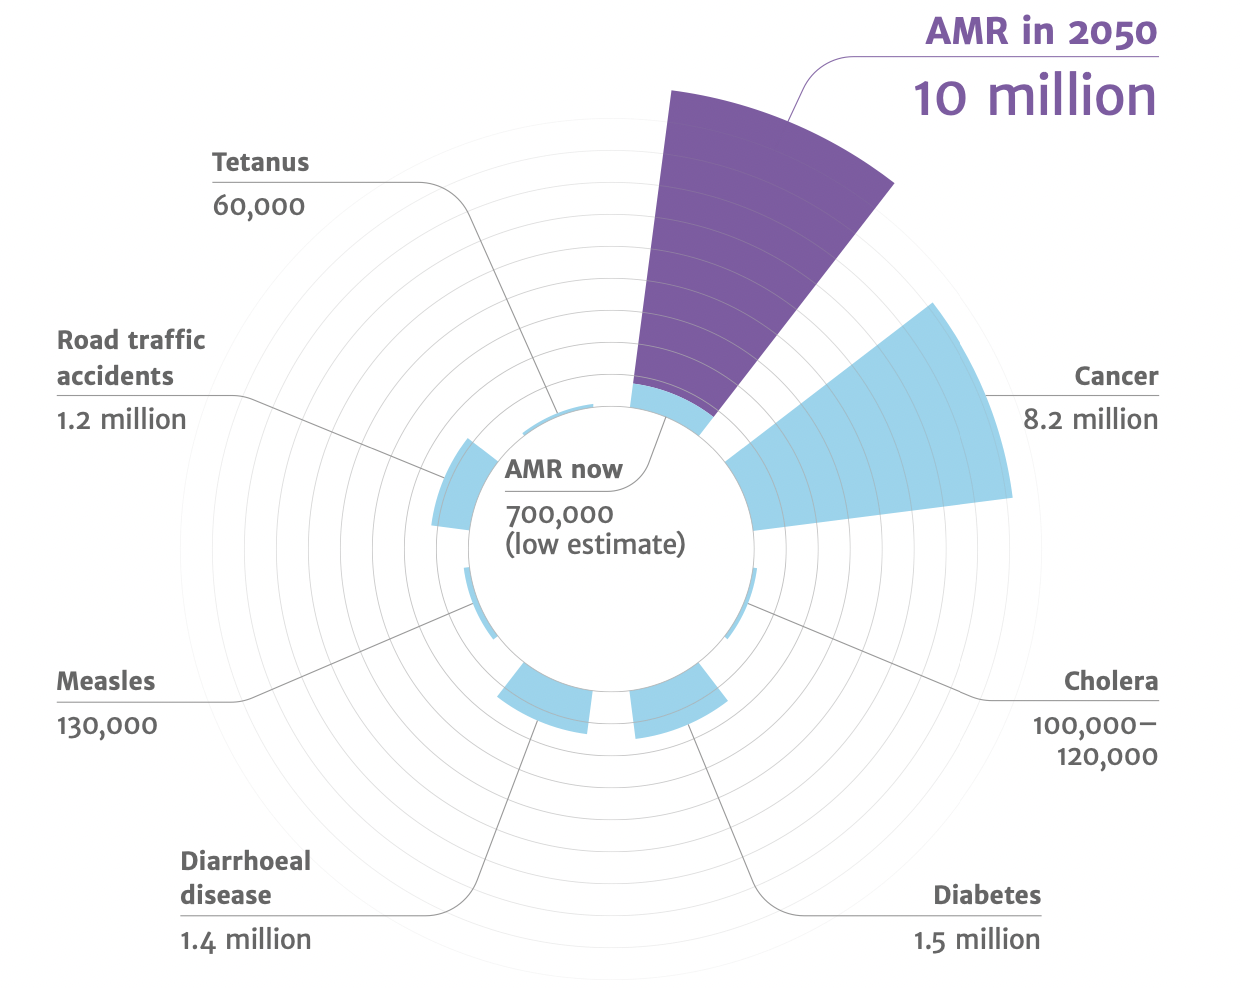
\includegraphics[height=0.8\textheight]{Figures/AMR_deaths.png}
\end{frame}
\begin{frame}{One Health approach to AMR}
	\centering
	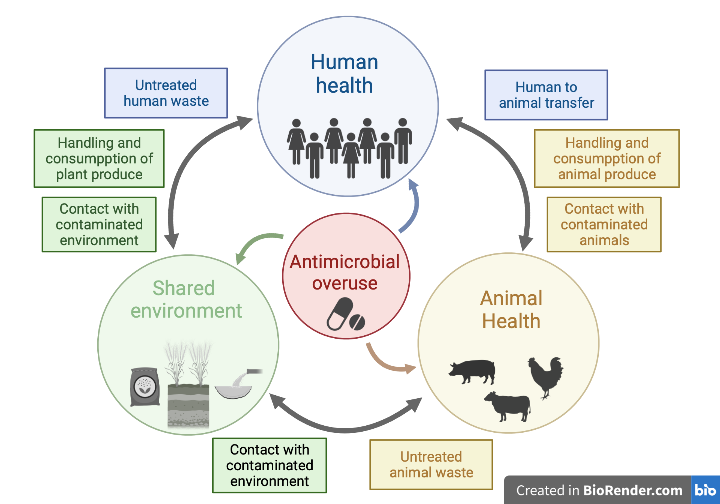
\includegraphics[width=0.9\textwidth]{Figures/One_health.png}
\end{frame}
\subsection{Project overview}
\begin{frame}{Our focus}
	\centering
	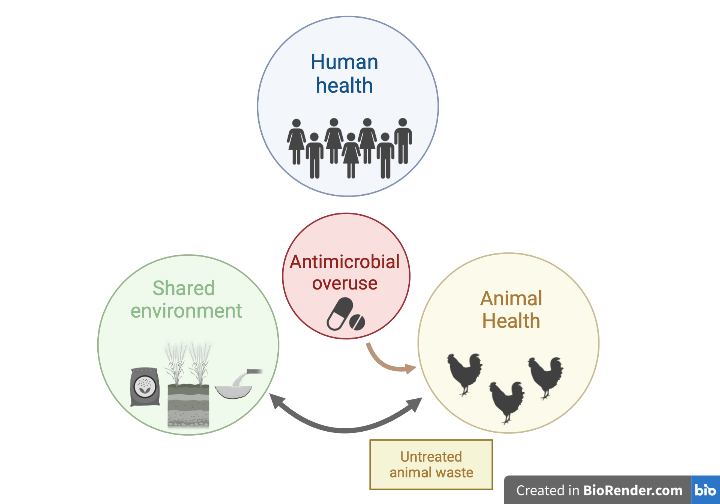
\includegraphics[width=0.9\textwidth]{Figures/Our_focus.png}
\end{frame}
\begin{frame}{Overview of the project}
	\vspace{0.5cm}
	\includegraphics<1>[width=0.9\textwidth]{Figures/project_overview.png}
	\includegraphics<2>[width=\textwidth]{Figures/project_modified.png}
\end{frame}
\begin{frame}{UoN team}
\centering
	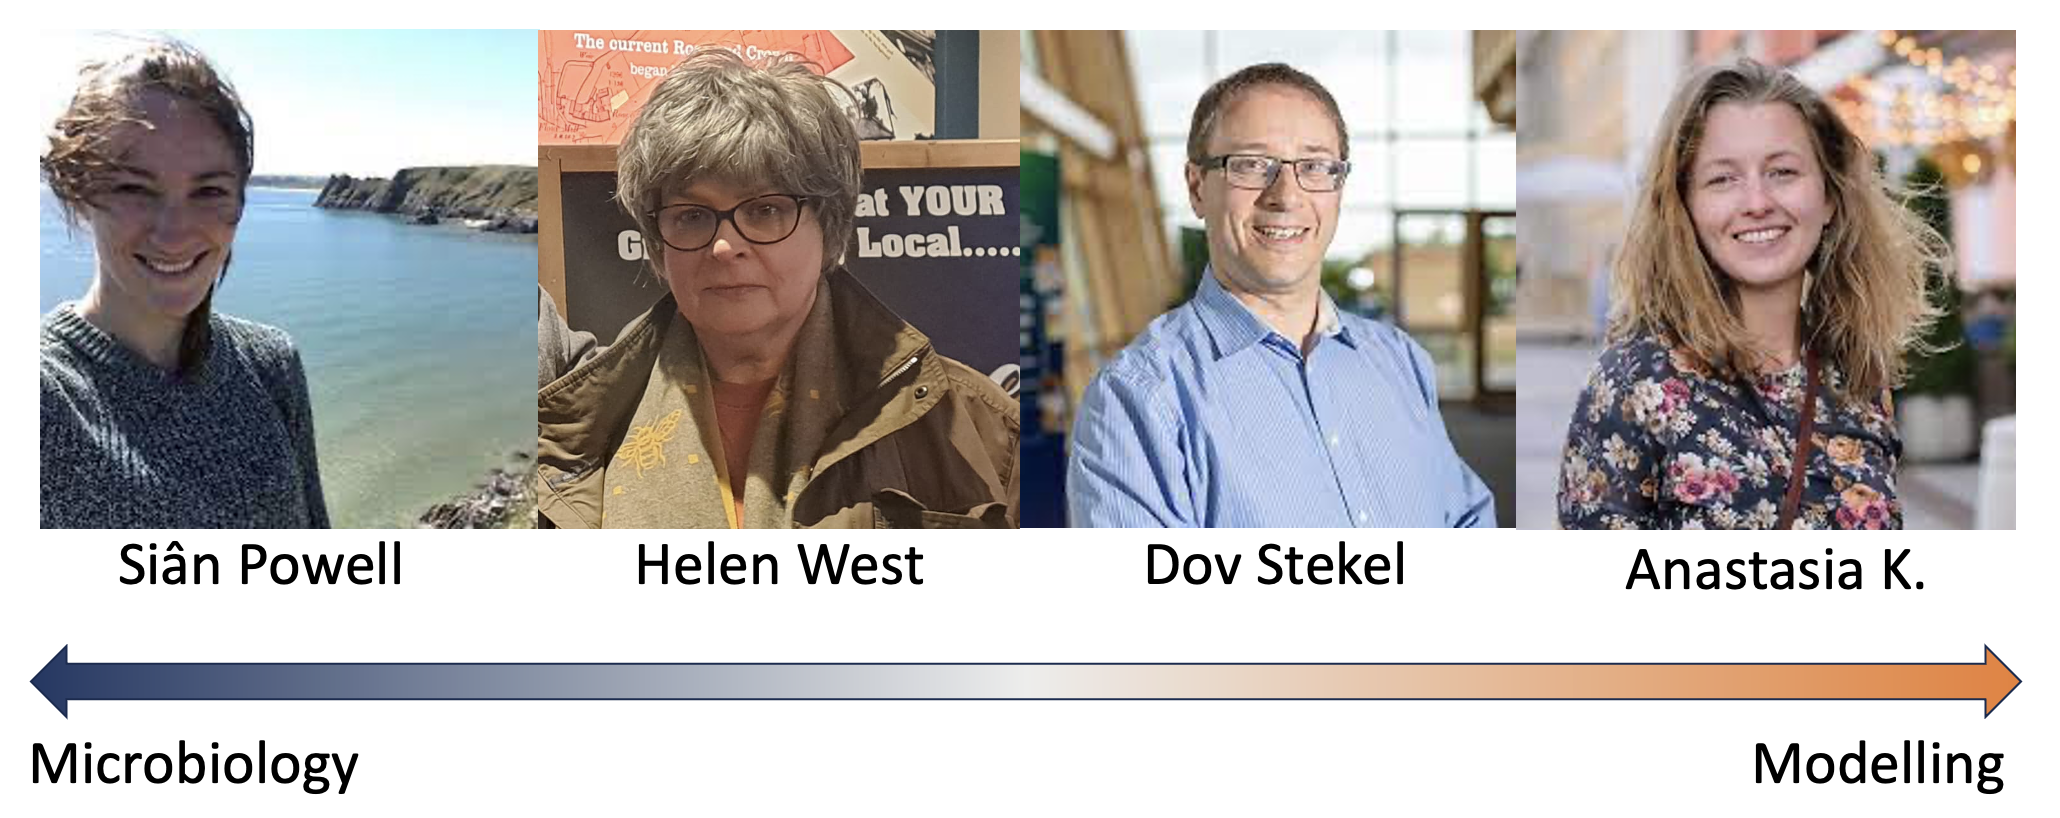
\includegraphics[width=\textwidth]{Figures/team_uon.png}\\
	\vspace{0.5cm}
	\only<1>{\textcolor{orange}{Our aim:} analyse and model the effect of composting on AMR in poultry manure.}
	\only<2>{\textcolor{orange}{Our  updated aim:} analyse and model the effect of composting on AMR in poultry manure \textbf{in absence of data.}}
\end{frame}
\begin{frame}{UoN research question}
\vspace{=-0.5cm}
	\includegraphics<1>[width=0.9\textwidth]{Figures/Compost-piles-new-farm.jpg}
	\includegraphics<2>[height=0.85\textheight]{Figures/heap_env.png}
	\includegraphics<3>[height=0.85\textheight]{Figures/heap_env_q.png}
\end{frame}
%%%%%%%%%%%%%%%%%%%%%%%%%%%%%%%%%%%%%%%%%%%%%%%%%%%%%%%%%%%%%%%%%%%%%%%%%%%%%%%%%%%%%%%%
\section{Basics of mathematical modelling}
\subsection{How we approximate reality}
\begin{frame}{What is a model?}
\centering
\begin{columns}
\begin{column}{0.5\textwidth}
\centering
		1. 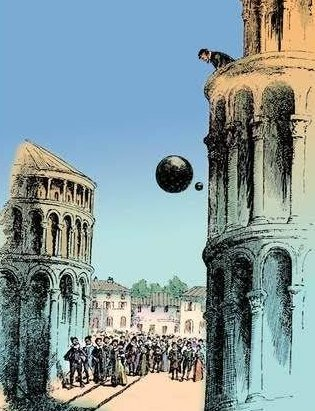
\includegraphics[width=0.7\textwidth]{Figures/galileo.jpg}\\
			3. 
\includegraphics[width=0.7\textwidth]{Figures/OpenAI_ChatGPT.png}\\
\end{column}
\begin{column}{0.5\textwidth}
\centering
	2.
\includegraphics[width=0.5\textwidth]{Figures/globe.jpg}\\
	\vspace{0.2cm}
		4. 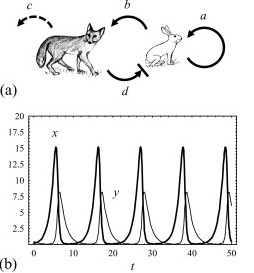
\includegraphics[width=0.7\textwidth]{Figures/lotka_voltera.jpg}\\
\end{column}
\end{columns}
\end{frame}
\begin{frame}{What is a mathematical model}
\centering
\begin{columns}
\begin{column}{0.5\textwidth}
\centering
\textcolor{orange}{Phenomenological \\(arise from first principles):}\\
\begin{itemize}
	\item Energy is conserved:
 \begin{align*}
		K_1 + U_1 = K_2 + U_2
	\end{align*}
	\item Action of  forces:
		\begin{align*}
		F = m a
	\end{align*}
	\item All things aim to reach equilibrium:
	\begin{align*}
			K_{eq} = \frac{\lbrack A\rbrack ^a \lbrack B\rbrack^b}{\lbrack C\rbrack^c \lbrack D\rbrack^d}
	\end{align*}
\end{itemize}
\end{column}
\begin{column}{0.5\textwidth}
\centering
\textcolor{purple}{Empirical(Data-driven):}\\
\begin{itemize}
	\item Lack interpretable structure
	\item Reveal hidden connections within data
	\item Predict system behaviour without understanding it
\end{itemize}
\centering
 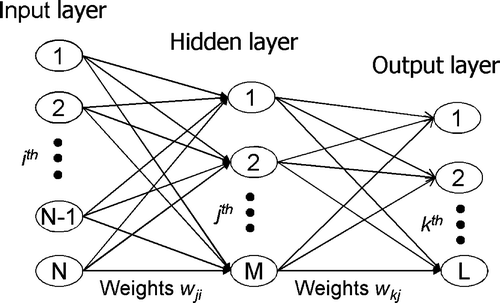
\includegraphics[width=\textwidth]{Figures/neunet.png}\\
\end{column}
\end{columns}
\end{frame}
\subsection{Model features}
\begin{frame}{What is a good model?}
We aim for these properties:\\
	\begin{itemize}
		\item \textbf{Predictive power and accuracy:} how closely can it replicate the real system.
		\item \textbf{Parsimony:} the simplest explanation is the most probable one.
		\item \textbf{Identifiability:} all model parameters can be uniquely determined from observing the real system.
		\item \textbf{Modular structure:} we want to add or remove model terms as our assumptions about the real system change
		\item \textbf{Validity:} model structure is "based in truth and reason", or model outputs can be compared with the system  behaviour for validation
		\end{itemize}
\end{frame}
\begin{frame}{What is a dynamical model?}
\centering
\begin{columns}
\begin{column}{0.3\textwidth}
\centering
\large Change of something in time, space, or both
\end{column}
\begin{column}{0.2\textwidth}
\centering
\LARGE 
= 
\end{column}
\begin{column}{0.5\textwidth}
\centering
\large
Forces, environmental aspects, concentrations governing change
\end{column}
\end{columns}
\vspace{0.3cm}
\visible<2->{\Large \textcolor{orange}{What interests us in a compost heap:}
\vspace{0.3cm}
\begin{columns}
\begin{column}{0.3\textwidth}
\centering
\large Change of \textbf{litter microbiome} in space and time
\end{column}
\begin{column}{0.2\textwidth}
\centering
\LARGE 
= 
\end{column}
\begin{column}{0.5\textwidth}
\centering
\large
Temperature and other environmental factors of the heap \& AMR
\end{column}
\end{columns}}
\visible<3->{
\vspace{0.3cm}
\begin{columns}
\begin{column}{0.3\textwidth}
\centering
\large Change of \textbf{litter temperature} in space and time
\end{column}
\begin{column}{0.2\textwidth}
\centering
\LARGE 
= 
\end{column}
\begin{column}{0.5\textwidth}
\centering
\large
Microbial activity and thermal fluxes
\end{column}
\end{columns}}
\end{frame}
%%%%%%%%%%%%%%%%%%%%%%%%%%%%%%%%%%%%%%%%%%%%%%%%%%%%%%%%%%%%%%%%%%%%%%%%%%%%%%%%%%%%%%%%
\section{First-principle modelling of compost heaps}
%%%%%%%%%%%%%%%%%%%%%%%%%%%%%%%%%%%%%%%%%%%%%%%%%%%%%%%%%%%%%%%%%%%%%%%%%%%%%%%%%%%%%%%%
\subsection{Primary model}
\begin{frame}{Principal variables}
\centering
	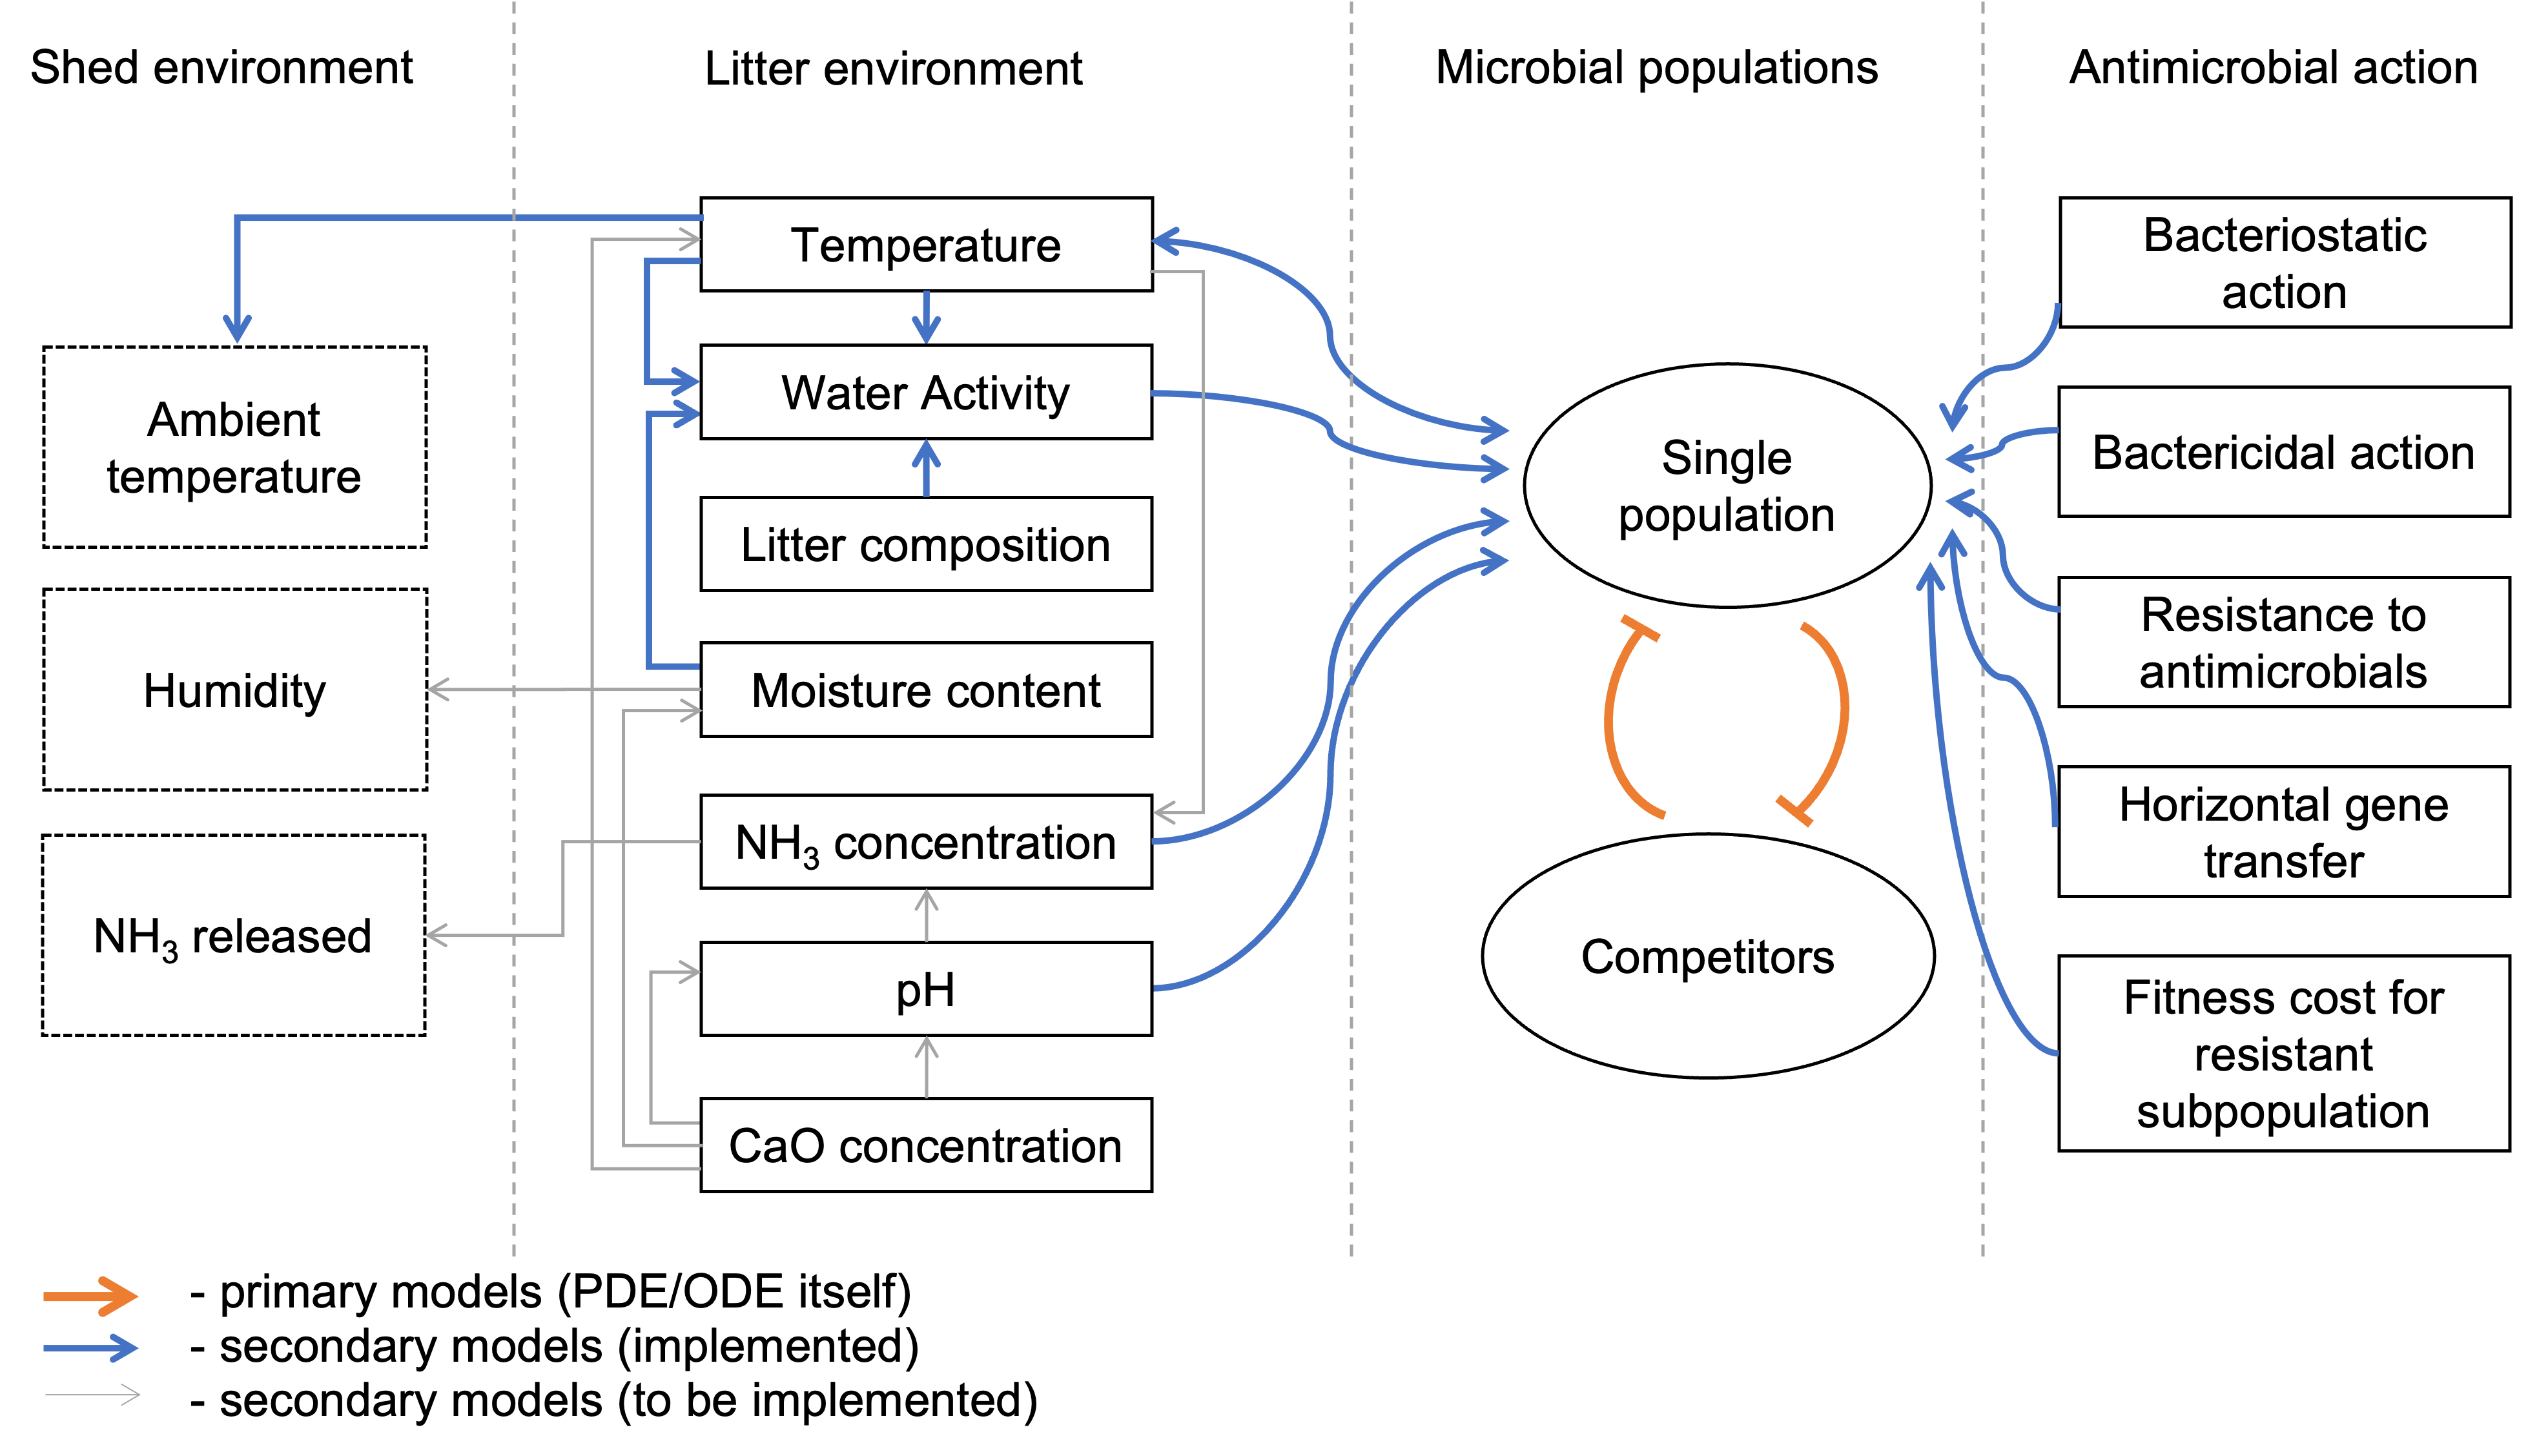
\includegraphics[width=0.92\textwidth]{Figures/variable_interaction.png}
\end{frame}
\begin{frame}{Measurable variables}
\centering
	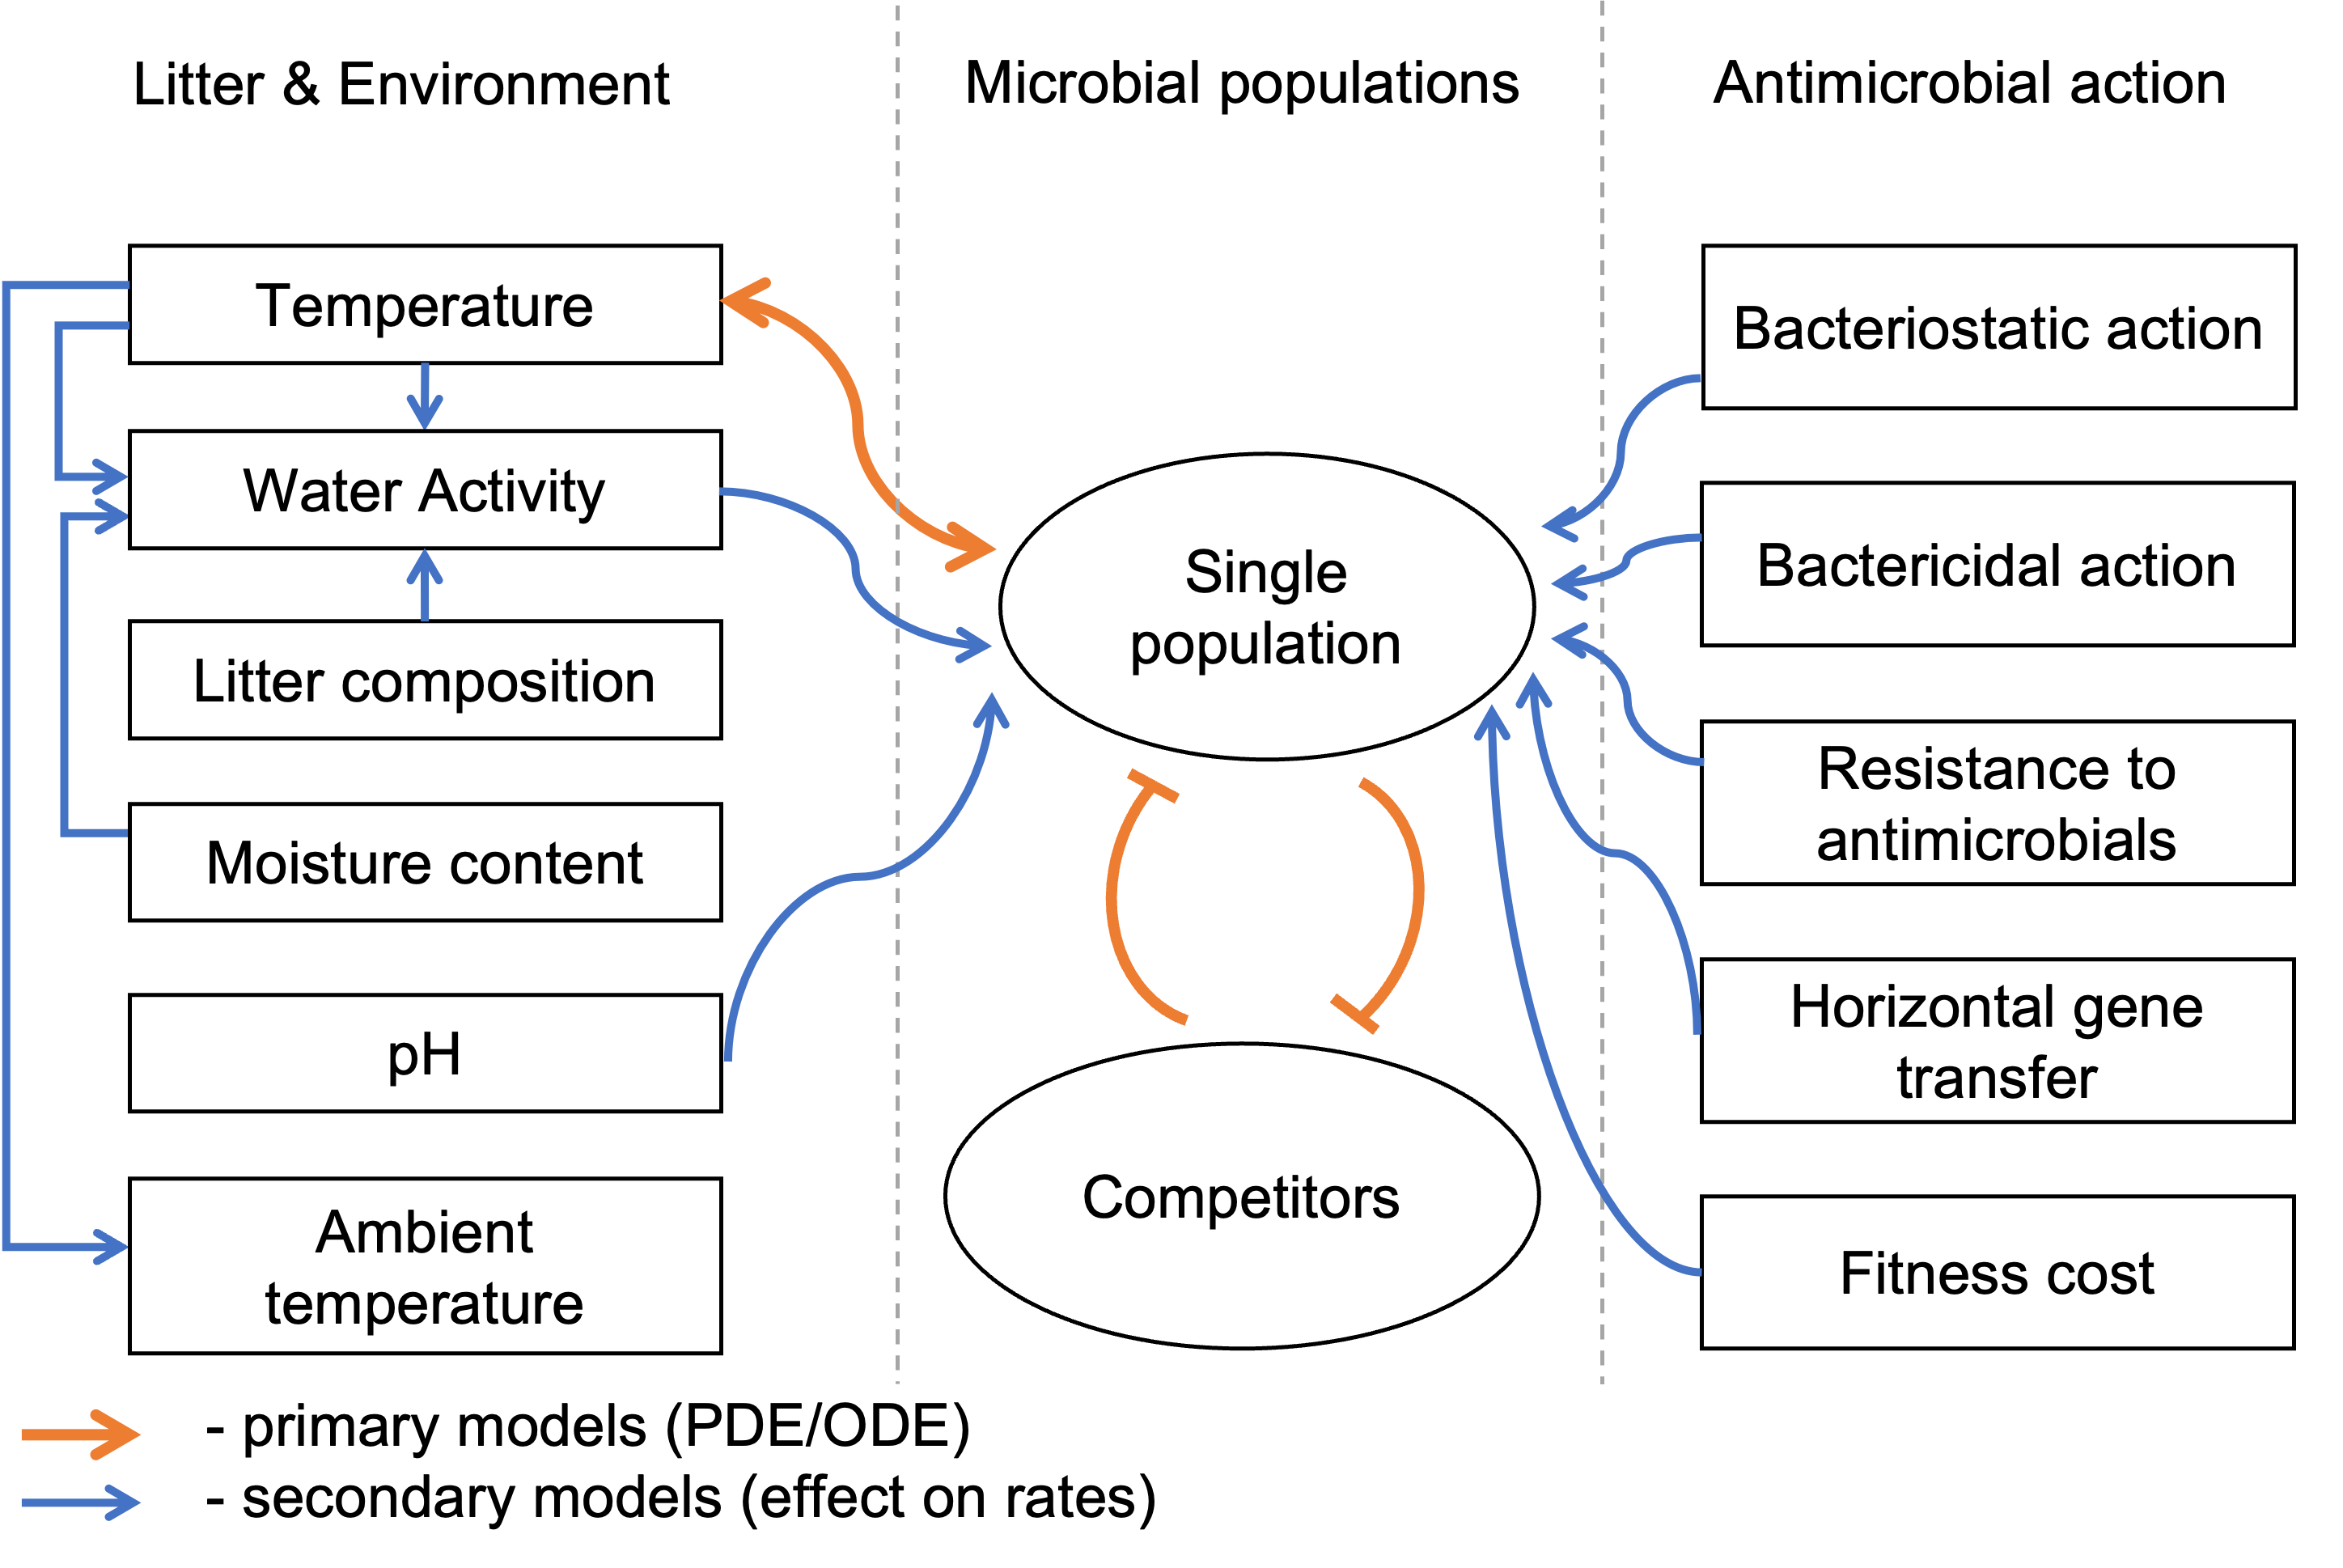
\includegraphics[width=0.78\textwidth]{Figures/variables_simple.png}
\end{frame}
\begin{frame}{Small prototype}
\begin{columns}
	\begin{column}{0.6\textwidth}
		Several species modelled as a closed system:\begin{itemize}
			\item \textit{Escherichia coli}
			\item \textit{Clostridium perfringens}
			\item \textit{Bacillus cereus} 
			\item \textit{Enterococcus faecium}
		\end{itemize}
		\vspace{0.5cm}
%		Self-heating process:
%				\begin{align*}
%\frac{\partial \mathrm{T}}{ \partial t} = \underbrace{D_{\mathrm{T}} \nabla \mathrm{T}}_{\text{heat diffusion}} + \underbrace{
% \sum_j \frac{(r_g)_j}{1 + (r_d)_j}r_{c,i} u_j}_{\text{microbial activity rate}}
%\end{align*}
	\end{column}
		\begin{column}{0.4\textwidth}
		 \definecolor{c1}{rgb}{0.2,0.4,0.6} % Blue-ish
\definecolor{c2}{rgb}{0.6,0.2,0.2} % Red-ish
\definecolor{c3}{rgb}{0.6,0.0,0.0} % Red
 \begin{tikzpicture}
  [tdplot_rotated_coords,
    scale=3,
    cube/.style={color=c1,thick,draw=gray, fill opacity=0.5,line join=round},
    mds/.style={ball color=c2, c2, opacity=.8},
    helplines/.style={gray,line cap=round},
    length/.style={<->,thick,line cap=round},
    axis/.style={->,c3,ultra thick,line cap=round},
    textlabel/.style={fill opacity=.7,text opacity=1,fill=white,rounded corners}]
  \def\d{1}
  \def\r{\d*.3}
  \def\af{\d*.5}
    % Draw backside of the cube
    \fill[cube] (0,0,\d) -- (0,\d,\d) -- (\d,\d,\d) -- (\d,0,\d) -- cycle;
    \fill[cube] (0,0,0) -- (0,0,\d) -- (\d,0,\d) -- (\d,0,0) -- cycle;
    \fill[cube] (\d,0,0) -- (\d,0,\d) -- (\d,\d,\d) -- (\d,\d,0) -- cycle;
    % Draw helplines
  \foreach \t in {0,12,...,348} % circle
    \draw[helplines] ({cos(\t   )*\r+\d/2}, \d/2, {sin(\t   )*\r+\d/2})
                      -- ({cos(\t+12)*\r+\d/2}, \d/2, {sin(\t+12)*\r+\d/2});
  \draw[helplines] (\d/2,\d/2-\r,\d/2) -- (\d/2,\d/2+\r,\d/2); % vertical line
    % Cylinder 
%  \shade[mds] (\d/2,\d/2,\d/2) circle (\r cm); % <= the little " cm" is needed to "trick" (?) everything into working...
    % Draw front of cube
    \fill[cube,fill=none] (0,0,0) -- (0,\d,0) -- (\d,\d,0) -- (\d,0,0) -- cycle;
    \fill[cube,fill=none] (0,\d,0) -- (0,\d,\d) -- (\d,\d,\d) -- (\d,\d,0) -- cycle;
    \fill[cube,fill=none] (0,0,0) -- (0,0,\d) -- (0,\d,\d) -- (0,\d,0) -- cycle;
    % Draw the axis arrows and annotations
    \draw[axis] (0,0,0) -- (\af,0,0) node[textlabel,anchor=east]{$x$};
    \draw[axis] (0,0,0) -- (0,\af,0) node[textlabel,anchor=south]{$y$};
    \draw[axis] (0,0,0) -- (0,0,\af) node[textlabel,anchor=west]{$z$};
%    % Draw radius arrow
%    \draw[mds,length,draw] (\d/2,\d/2,\d/2) -- (\d/2,\d/2,\d/2-\r) node[textlabel,pos=0.5, auto=above]{$r$};
    % Draw cube lattice length measures
    \draw[cube,length,c1] (0,0,\d*5/6) -- (0,\d,\d*5/6) node[textlabel,pos=0.5, auto=above]{$d$};
    \draw[cube,length,c1] (\d*5/6,0,0) -- (\d*5/6,\d,0) node[textlabel,pos=0.5, auto=above]{$d$};
    \draw[cube,length,c1] (\d*5/6,\d,0) -- (\d*5/6,\d,\d) node[textlabel,pos=0.5, auto=above]{$d$};   
\end{tikzpicture}
		\end{column}
	\end{columns}
\end{frame}
\begin{frame}{Population dynamics}
		 Rate of change of an individual population (taxon) at point $\mathbf{s}$:
	\begin{align*}\label{eq:simple_diff}
\frac{\partial u}{ \partial t} = \underbrace{ D \nabla u}_{\text{redistribution}} +
 \underbrace{r_{g}(t, \mathbf{s}, \xi) \left(\frac{K_{max} - u - v}{K_{max}} \right) u}_{\text{growth}} - \underbrace{r_{d}(t, \mathbf{s}, \xi) u}_{\text{death}} + \underbrace{r_{HGT} v}_{\text{HGT}},	
\end{align*}
\begin{itemize}
	\item $u$ - population size (abundance);
	\item $v$ - co-inhabiting population size (abundance);
	\item $K_{max}$ - carrying capacity of the environment;
	\item $D$ - diffusion rate;
	\item $r_{g}(t, \mathbf{s}, \xi), r_{d}(t, \mathbf{s}, \xi)$ - spatiotemporally changing growth and death rates;
	\item $\xi = \lbrace \mathrm{T}, \mathrm{pH}, a_w \rbrace$ - environmental factors (temperature, pH, water activity, AMR-related fitness costs).
\end{itemize}
\end{frame}
%%%%%%%%%%%%%%%%%%%%%%%%%%%%%%%%%%%%%%%%%%%%%%%%%%%%%%%%%%%%%%%%%%%%%%%%%%%%%%%%%%%%%%%%
\subsection{Secondary models}
\begin{frame}{Growth modelling}
From \cite{Zwietering1992}, optimal growth rate is inhibited by independent factors:
	\begin{align*}
		r_g = r_{opt} \gamma(\mathrm{\mathrm{T}}) \gamma(\mathrm{pH}) \gamma(a_w),
	\end{align*}
	where from \cite{Rosso1993}:
	\begin{align*}
	\gamma(\mathrm{T}) = \frac{(\mathrm{T} - \mathrm{T}_{max})(\mathrm{T} - \mathrm{T}_{min})^2}{(\mathrm{T} - \mathrm{T}_{min})(\mathrm{T} - \mathrm{T}_{max}) - (\mathrm{T} - \mathrm{T}_{opt})^2}
	\end{align*}
	from \cite{Akkermans2018}:
	\begin{align*}
	\gamma(\mathrm{pH}) = \frac{(\mathrm{pH} - \mathrm{pH}_{max})(\mathrm{pH} - \mathrm{pH}_{min})^2}{(\mathrm{pH} - \mathrm{pH}_{min})(\mathrm{pH} - \mathrm{pH}_{max}) - (\mathrm{pH} - \mathrm{pH}_{opt})^2}
	\end{align*}
	from \cite{McMeekin1987}:
	\begin{align*}
	\gamma(a_w) = \frac{(a_w - a_{min})}{(1 - a_{min})}
	\end{align*}
\end{frame}
\begin{frame}{Growth inhibiting factors}
Growth rates at optimal conditions for each population are taken from ComBase broth models.\\
Cardinal temperatures, pH, water activity are taken form literature:\\
\centering
	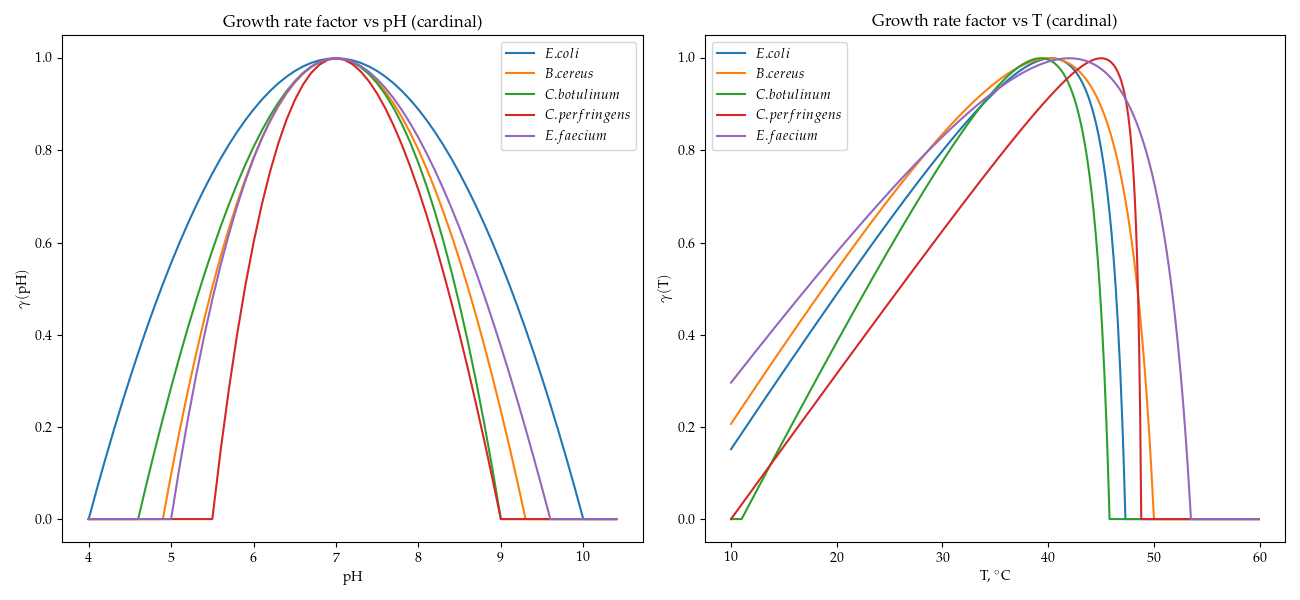
\includegraphics[width=0.9\textwidth]{Figures/inhibiting_factors_growth}
\end{frame}
\begin{frame}{Water activity}
	A data-driven model is available for chicken litter with pine shavings \cite{Hendriks2014}:\\
	\centering
	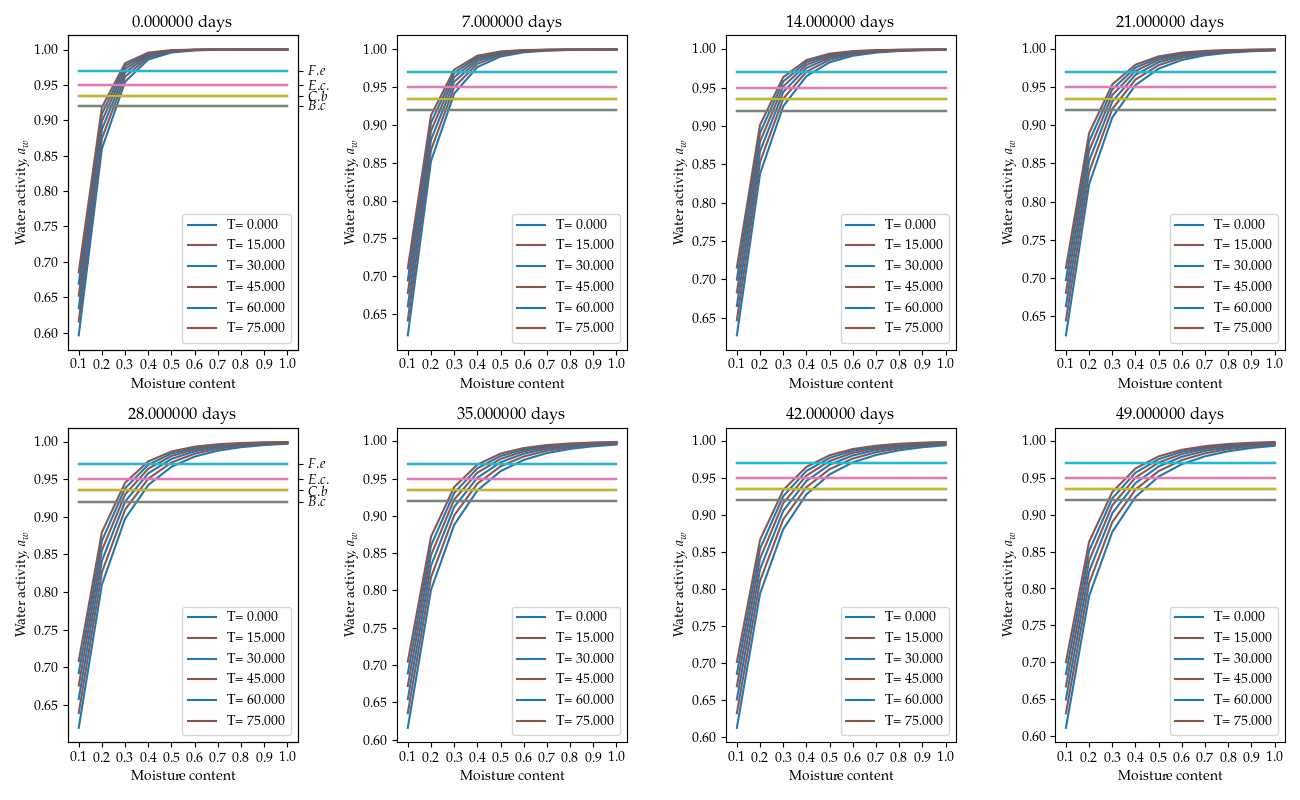
\includegraphics[width=0.9\textwidth]{Figures/aw_vs_moisture}
\end{frame}
\begin{frame}{Model of self-heating}
Self-heating process is reflected in the temperature model as proportional to total growth of biota:
	\begin{align*}
\frac{\partial T}{ \partial t} = \nabla D \nabla T +
 \sum_j \frac{(r_g)_j}{1 + (r_d)_j}r_{c,i} \left(\frac{K_{max} - u_j - \sum_i \upsilon_i}{K_{max}} \right) u_j 
% - r_{rad}f(T - T_{air}) - r_{conv}f(T - T_{soil}),
\end{align*}
\begin{itemize}
	\item Accounts for both activation and inactivation of microbial populations;
	\item Radiative and convective fluxes on the boundary can be turned on and off;
	\item Original model uses Arrhenius rate models, we plug in empirical models from literature.
\end{itemize}
\end{frame}
\begin{frame}{Defining assumptions}
\begin{itemize}
	\item N - the number of subpopulations of microbiome - is "relatively" small.
	\item Competition is actualised via the shared carrying capacity.
	\item For many species, we can take $\mathrm{T}_{min}, \mathrm{T}_{max}, \mathrm{T}_{opt}$ , $\mathrm{pH}{min}, \mathrm{pH}_{max}, \mathrm{pH}_{opt}$, and $a_{w0}$ from ComBase or literature.
	\item Temperature only changes due to microbial activity, diffusion, and radiative flux to the environment.
	\item Unknown parameters: $D_{\mathrm{T}}, r_{\mathrm{T},rad}, K_max$ and for each subpopulaition $D, r_g, r_d, r_{HGT}, \gamma_{res,1}, \dots, \gamma_{res,M}$, where M is number of detected resistances.
	\item Total 3 + N*(4+M) unknown model parameters. 
\end{itemize}
\end{frame}
\subsection{Prototype in action}
\begin{frame}{3D simulation of a self-heating compost heap}
	\centering
\animategraphics[loop,width=11cm]{10}{Figures/sh}{1}{122}	
\end{frame}
\section{Reality check}
\begin{frame}{Expanded prototype}
\begin{columns}
	\begin{column}{0.6\textwidth}
		Several species modelled as a closed system:\begin{itemize}
			\item \textit{Escherichia coli}
			\item \textit{Clostridium perfringens}
			\item \textit{Bacillus cereus} 
			\item \textit{Enterococcus faecium}
			\item \textcolor{orange}{the rest!}
		\end{itemize}
		\vspace{0.5cm}
%		Self-heating process:
%				\begin{align*}
%\frac{\partial \mathrm{T}}{ \partial t} = \underbrace{D_{\mathrm{T}} \nabla \mathrm{T}}_{\text{heat diffusion}} + \underbrace{
% \sum_j \frac{(r_g)_j}{1 + (r_d)_j}r_{c,i} u_j}_{\text{microbial activity rate}}
%\end{align*}
	\end{column}
		\begin{column}{0.4\textwidth}
		 \definecolor{c1}{rgb}{0.2,0.4,0.6} % Blue-ish
\definecolor{c2}{rgb}{0.6,0.2,0.2} % Red-ish
\definecolor{c3}{rgb}{0.6,0.0,0.0} % Red
 \begin{tikzpicture}
  [tdplot_rotated_coords,
    scale=3,
    cube/.style={color=c1,thick,draw=gray, fill opacity=0.5,line join=round},
    mds/.style={ball color=c2, c2, opacity=.8},
    helplines/.style={gray,line cap=round},
    length/.style={<->,thick,line cap=round},
    axis/.style={->,c3,ultra thick,line cap=round},
    textlabel/.style={fill opacity=.7,text opacity=1,fill=white,rounded corners}]
  \def\d{1}
  \def\r{\d*.3}
  \def\af{\d*.5}
    % Draw backside of the cube
    \fill[cube] (0,0,\d) -- (0,\d,\d) -- (\d,\d,\d) -- (\d,0,\d) -- cycle;
    \fill[cube] (0,0,0) -- (0,0,\d) -- (\d,0,\d) -- (\d,0,0) -- cycle;
    \fill[cube] (\d,0,0) -- (\d,0,\d) -- (\d,\d,\d) -- (\d,\d,0) -- cycle;
    % Draw helplines
  \foreach \t in {0,12,...,348} % circle
    \draw[helplines] ({cos(\t   )*\r+\d/2}, \d/2, {sin(\t   )*\r+\d/2})
                      -- ({cos(\t+12)*\r+\d/2}, \d/2, {sin(\t+12)*\r+\d/2});
  \draw[helplines] (\d/2,\d/2-\r,\d/2) -- (\d/2,\d/2+\r,\d/2); % vertical line
    % Cylinder 
%  \shade[mds] (\d/2,\d/2,\d/2) circle (\r cm); % <= the little " cm" is needed to "trick" (?) everything into working...
    % Draw front of cube
    \fill[cube,fill=none] (0,0,0) -- (0,\d,0) -- (\d,\d,0) -- (\d,0,0) -- cycle;
    \fill[cube,fill=none] (0,\d,0) -- (0,\d,\d) -- (\d,\d,\d) -- (\d,\d,0) -- cycle;
    \fill[cube,fill=none] (0,0,0) -- (0,0,\d) -- (0,\d,\d) -- (0,\d,0) -- cycle;
    % Draw the axis arrows and annotations
    \draw[axis] (0,0,0) -- (\af,0,0) node[textlabel,anchor=east]{$x$};
    \draw[axis] (0,0,0) -- (0,\af,0) node[textlabel,anchor=south]{$y$};
    \draw[axis] (0,0,0) -- (0,0,\af) node[textlabel,anchor=west]{$z$};
%    % Draw radius arrow
%    \draw[mds,length,draw] (\d/2,\d/2,\d/2) -- (\d/2,\d/2,\d/2-\r) node[textlabel,pos=0.5, auto=above]{$r$};
    % Draw cube lattice length measures
    \draw[cube,length,c1] (0,0,\d*5/6) -- (0,\d,\d*5/6) node[textlabel,pos=0.5, auto=above]{$d$};
    \draw[cube,length,c1] (\d*5/6,0,0) -- (\d*5/6,\d,0) node[textlabel,pos=0.5, auto=above]{$d$};
    \draw[cube,length,c1] (\d*5/6,\d,0) -- (\d*5/6,\d,\d) node[textlabel,pos=0.5, auto=above]{$d$};   
\end{tikzpicture}
		\end{column}
	\end{columns}
\end{frame}
%\subsection{Expanded prototype in action}
%\begin{frame}{3D simulation of a self-heating compost heap}
%	\centering
%\animategraphics[loop,width=11cm]{10}{Figures/sh}{1}{122}	
%\end{frame}
\begin{frame}{Is our model good?}
\vspace{0.5cm}
	\begin{itemize}
		\item<1-> \textbf{Predictive power and accuracy:} we don't know because there is no data to compare it with.
		\item<2-> \textbf{\textcolor{green}{Parsimony:}} we include the basic processes related to measurable variables.
		\item<3-> \textbf{\textcolor{magenta}{Identifiability:}} a lot of confounding factors and model terms.
		\item<4->  \textbf{\textcolor{green}{Modular structure:}} can easily expand or reduce the number of populations, environmental effects on the populations.
		\item<5-> \textbf{\textcolor{green}{Validity:}} we employ established approximations derived from data or validated by experiments in the literature. Outputs directly related to measured variables. 
	\end{itemize}
\end{frame}
\begin{frame}{Interlude}
	How we can modify the model:
	\begin{itemize}
		\item Add mode populations
		\item Add other environmental factors via rate inhibitors
		\item Change boundary conditions for the temperature to simulate insulated piles, convective vs radioative heat transfer
		\item Change parametrisation of growth and death rates.
	\end{itemize}
\end{frame}
%%%%%%%%%%%%%%%%%%%%%%%%%%%%%%%%%%%%%%%%%%%%%%%%%%%%%%%%%%%%%%%%%%%%%%%%%%%%%%%%%%%%%%%%
\section<presentation>*{Appendix}
\subsection<presentation>*{References}
\begin{frame}[allowframebreaks]
\printbibliography
\end{frame}
\begin{frame}
\centering
\Huge{Thank you!}\\
\huge{Questions?}
\end{frame}
\subsection{The question of Death}
\begin{frame}{Thermal inactivation modelling}
\begin{itemize}
	\item Very few models consider non-isothermic treatment of bacteria.
	\item Cerf model \cite{Cerf1996} links death rate to the environment:
	\begin{align*}
		\log{r_d} = C_0 + C_1 / \mathrm{T} + C_2 \mathrm{pH} + C_2 \mathrm{pH}^2 + C_4 (a_w)^2,
	\end{align*}
	where $C_0, \dots C_4$ must be estimated for each species.
	\item Majority of others rely on inactivation time \cite{GAILLARD1998}:
	\begin{align*}
		\log(D) = \log_{10}(D^{\ast}) - \frac{1}{z_{\mathrm{T}}}(\mathrm{T} - \mathrm{T}^{\ast}) - \frac{1}{z_{\mathrm{pH}}}(\mathrm{pH} - \mathrm{pH}^{\ast}) - \frac{1}{z_{a_w}}(a_w - 1)
	\end{align*}
	where $z_{\mathrm{T}}, z_{\mathrm{pH}}, z_{a_w}$ must be estimated for each species.
	\item Relationship between rate and D-value: $D = \frac{\log(10)}{r_d}$.
\end{itemize} 
\end{frame}
\begin{frame}{Thermal inactivation rates}
\textit{Escherichia coli} model from \cite{Cerf1996}, \textit{Bacillus cereus} model from \cite{GAILLARD1998}. For others model coefficients from \cite{GAILLARD1998} are corrected to account for known behaviour:\\
\centering
	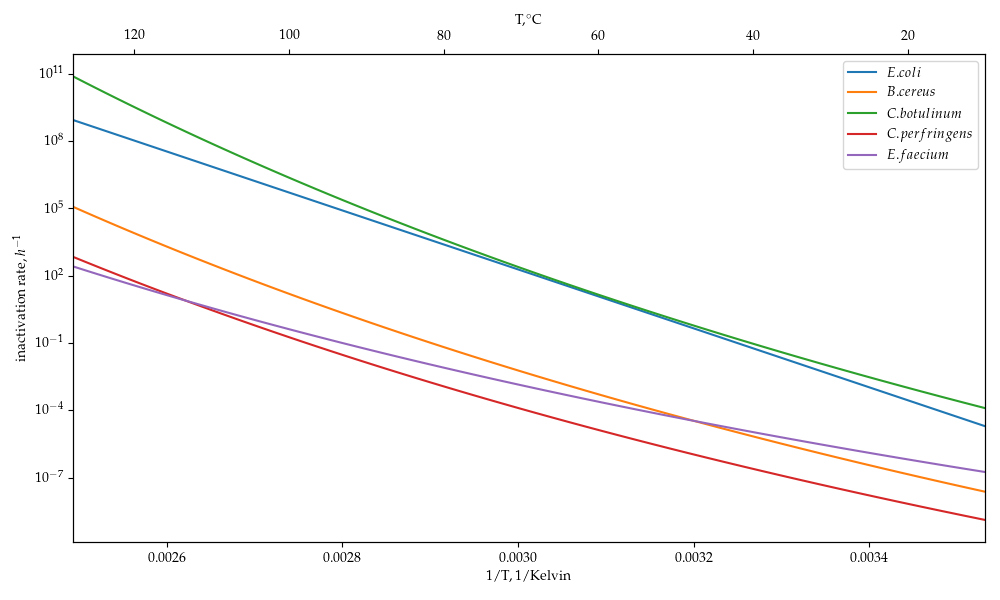
\includegraphics[width=0.9\textwidth]{Figures/Cerf_death_rates.png}
\end{frame}
\end{document}